\documentclass[final]{beamer}\usepackage[]{graphicx}\usepackage[]{color}
%% maxwidth is the original width if it is less than linewidth
%% otherwise use linewidth (to make sure the graphics do not exceed the margin)
\makeatletter
\def\maxwidth{ %
  \ifdim\Gin@nat@width>\linewidth
    \linewidth
  \else
    \Gin@nat@width
  \fi
}
\makeatother

\definecolor{fgcolor}{rgb}{0.345, 0.345, 0.345}
\newcommand{\hlnum}[1]{\textcolor[rgb]{0.686,0.059,0.569}{#1}}%
\newcommand{\hlstr}[1]{\textcolor[rgb]{0.192,0.494,0.8}{#1}}%
\newcommand{\hlcom}[1]{\textcolor[rgb]{0.678,0.584,0.686}{\textit{#1}}}%
\newcommand{\hlopt}[1]{\textcolor[rgb]{0,0,0}{#1}}%
\newcommand{\hlstd}[1]{\textcolor[rgb]{0.345,0.345,0.345}{#1}}%
\newcommand{\hlkwa}[1]{\textcolor[rgb]{0.161,0.373,0.58}{\textbf{#1}}}%
\newcommand{\hlkwb}[1]{\textcolor[rgb]{0.69,0.353,0.396}{#1}}%
\newcommand{\hlkwc}[1]{\textcolor[rgb]{0.333,0.667,0.333}{#1}}%
\newcommand{\hlkwd}[1]{\textcolor[rgb]{0.737,0.353,0.396}{\textbf{#1}}}%
\let\hlipl\hlkwb

\usepackage{framed}
\makeatletter
\newenvironment{kframe}{%
 \def\at@end@of@kframe{}%
 \ifinner\ifhmode%
  \def\at@end@of@kframe{\end{minipage}}%
  \begin{minipage}{\columnwidth}%
 \fi\fi%
 \def\FrameCommand##1{\hskip\@totalleftmargin \hskip-\fboxsep
 \colorbox{shadecolor}{##1}\hskip-\fboxsep
     % There is no \\@totalrightmargin, so:
     \hskip-\linewidth \hskip-\@totalleftmargin \hskip\columnwidth}%
 \MakeFramed {\advance\hsize-\width
   \@totalleftmargin\z@ \linewidth\hsize
   \@setminipage}}%
 {\par\unskip\endMakeFramed%
 \at@end@of@kframe}
\makeatother

\definecolor{shadecolor}{rgb}{.97, .97, .97}
\definecolor{messagecolor}{rgb}{0, 0, 0}
\definecolor{warningcolor}{rgb}{1, 0, 1}
\definecolor{errorcolor}{rgb}{1, 0, 0}
\newenvironment{knitrout}{}{} % an empty environment to be redefined in TeX

\usepackage{alltt}
\usepackage{graphicx}
\usepackage{color}
\usepackage{amsmath}
\usepackage{epstopdf}
\usepackage{multicol}
%% maxwidth is the original width if it is less than linewidth
%% otherwise use linewidth (to make sure the graphics do not exceed the margin)
\makeatletter
\def\maxwidth{ %
  \ifdim\Gin@nat@width>\linewidth
    \linewidth
  \else
    \Gin@nat@width
  \fi
}
\makeatother

\definecolor{fgcolor}{rgb}{0.345, 0.345, 0.345}
\newcommand{\hlnum}[1]{\textcolor[rgb]{0.686,0.059,0.569}{#1}}%
\newcommand{\hlstr}[1]{\textcolor[rgb]{0.192,0.494,0.8}{#1}}%
\newcommand{\hlcom}[1]{\textcolor[rgb]{0.678,0.584,0.686}{\textit{#1}}}%
\newcommand{\hlopt}[1]{\textcolor[rgb]{0,0,0}{#1}}%
\newcommand{\hlstd}[1]{\textcolor[rgb]{0.345,0.345,0.345}{#1}}%
\newcommand{\hlkwa}[1]{\textcolor[rgb]{0.161,0.373,0.58}{\textbf{#1}}}%
\newcommand{\hlkwb}[1]{\textcolor[rgb]{0.69,0.353,0.396}{#1}}%
\newcommand{\hlkwc}[1]{\textcolor[rgb]{0.333,0.667,0.333}{#1}}%
\newcommand{\hlkwd}[1]{\textcolor[rgb]{0.737,0.353,0.396}{\textbf{#1}}}%
\let\hlipl\hlkwb

\usepackage{framed}
\makeatletter
\newenvironment{kframe}{%
 \def\at@end@of@kframe{}%
 \ifinner\ifhmode%
  \def\at@end@of@kframe{\end{minipage}}%
  \begin{minipage}{\columnwidth}%
 \fi\fi%
 \def\FrameCommand##1{\hskip\@totalleftmargin \hskip-\fboxsep
 \colorbox{shadecolor}{##1}\hskip-\fboxsep
     % There is no \\@totalrightmargin, so:
     \hskip-\linewidth \hskip-\@totalleftmargin \hskip\columnwidth}%
 \MakeFramed {\advance\hsize-\width
   \@totalleftmargin\z@ \linewidth\hsize
   \@setminipage}}%
 {\par\unskip\endMakeFramed%
 \at@end@of@kframe}
\makeatother

\definecolor{shadecolor}{rgb}{.97, .97, .97}
\definecolor{messagecolor}{rgb}{0, 0, 0}
\definecolor{warningcolor}{rgb}{1, 0, 1}
\definecolor{errorcolor}{rgb}{1, 0, 0}
\newenvironment{knitrout}{}{} % an empty environment to be redefined in TeX

\usepackage{alltt}
\usepackage{grffile}
\mode<presentation>{\usetheme{CambridgeUSPOL}}

\usepackage[utf8]{inputenc}
\usepackage{amsfonts}
\usepackage{amsmath}
\usepackage{natbib}
% \usepackage{polski}
\usepackage{graphicx}
\usepackage{array,booktabs,tabularx}
\usepackage{epstopdf}
\usepackage[dvipsnames]{xcolor}
\usepackage{colortbl}
\newcolumntype{Z}{>{\centering\arraybackslash}X}

% rysunki
\usepackage{tikz}
\usepackage{ifthen}
\usepackage{xxcolor}
\usetikzlibrary{arrows}
\usetikzlibrary[topaths]
\usetikzlibrary{decorations.pathreplacing}
%\usepackage{times}\usefonttheme{professionalfonts}  % times is obsolete
\usefonttheme[onlymath]{serif}
\boldmath
\usepackage[orientation=portrait,size=a0,scale=1.4,debug]{beamerposter}                       % e.g. for DIN-A0 poster
%\usepackage[orientation=portrait,size=a1,scale=1.4,grid,debug]{beamerposter}                  % e.g. for DIN-A1 poster, with optional grid and debug output
%\usepackage[size=custom,width=200,height=120,scale=2,debug]{beamerposter}                     % e.g. for custom size poster
%\usepackage[orientation=portrait,size=a0,scale=1.0,printer=rwth-glossy-uv.df]{beamerposter}   % e.g. for DIN-A0 poster with rwth-glossy-uv printer check
% ...
%

\definecolor{red1}{RGB}{254,240,217}
\definecolor{red2}{RGB}{253,204,138}
\definecolor{red3}{RGB}{252,141,89}
\definecolor{red4}{RGB}{227,74,51}
\definecolor{red5}{RGB}{179,0,0}
\definecolor{MethanoGram}{RGB}{199, 55, 163}
\usecolortheme{seagull}
\useinnertheme{rectangles}
\setbeamercolor{item projected}{bg=darkred}
% \setbeamertemplate{enumerate items}[default]
\setbeamertemplate{caption}{\insertcaption} 
\setbeamertemplate{navigation symbols}{}
\setbeamercovered{transparent}
\setbeamercolor{block title}{fg=white,bg=MethanoGram}
\setbeamercolor{block body}{fg=black,bg=white}
\setbeamercolor{local structure}{fg=darkred}

\setbeamercolor*{enumerate item}{fg=darkred}
\setbeamercolor*{enumerate subitem}{fg=darkred}
\setbeamercolor*{enumerate subsubitem}{fg=darkred}

\setbeamercolor*{itemize item}{fg=darkred}
\setbeamercolor*{itemize subitem}{fg=darkred}
\setbeamercolor*{itemize subsubitem}{fg=darkred}

\newlength{\columnheight}
\setlength{\columnheight}{85cm}
\renewcommand{\thetable}{}
\def\andname{,}
\authornote{}

\renewcommand{\APACrefatitle}[2]{}
\renewcommand{\bibliographytypesize}{\footnotesize} 
\renewcommand{\APACrefYearMonthDay}[3]{%
  {\BBOP}{#1}
  {\BBCP}
}
\IfFileExists{upquote.sty}{\usepackage{upquote}}{}
\IfFileExists{upquote.sty}{\usepackage{upquote}}{}
\begin{document}




\date{}
\author{\large Micha\l{} Burdukiewicz\inst{1}, Przemys\l{}aw Gagat\inst{1}, S\l{}awomir Jab\l{}o\n{}ski\inst{2}, \underline{Jaros\l{}aw Chilimoniuk}\inst{1}, Micha\l{} Gaworski\inst{2}, \\ Pawe\l{} Mackiewicz\inst{1} and Marcin \L{}ukaszewicz\inst{2}*\\
\smallskip
\normaltext{*marcin.lukaszewicz@uwr.edu.pl}}
\institute{\small{\textsuperscript{1}University of Wroc\l{}aw, Department of Genomics,
\textsuperscript{2}University of Wroc\l{}aw, Department of Biotransformation
}
}

%Computational and experimental validation of amyloid databases
%Problems with annotation and computational prediction of peptide amyloidogenicity
\title{\huge PhyMet^2$: complex database containing records on methanogens with unique feature (MethanoGram) allowing prediction of culture conditions based on 16S rRNA}


\begin{frame}
\begin{columns}
\begin{column}{.53\textwidth}
\begin{beamercolorbox}[center,wd=\textwidth]{postercolumn}
\begin{minipage}[T]{.95\textwidth}
\parbox[t][\columnheight]{\textwidth}
{
\begin{block}{Introduction}

Methanogens are methane-producing anaerobic archaea, that can be found in many anaerobic habitats. They are recognized as the largest biogenic source of methane, which is a potent greenhouse gas, and consequently as an important factor in the global carbon cycle. They also show growing potential for biotechnological uses.\\ 
Our rudimentary knowledge about them results from difficulties with their isolation and culturing in laboratory conditions, which are necessary to describe their phenotype. Innovations in DNA sequencing technologies allowed for rapid development of metagenomics. DNA sequencing of environmental samples resulted in identifying a plethora of new uncultivated methanogens. \\
Therefore, we created PhyMet^2$, the first database that combines description of methanogens and their culturing conditions with genetic information.

\end{block}

\begin{block}{Data collection}

PhyMet2 contains 153 manually curated and up-to-date high quality records of methanogenic species. \\
Sequence data was collected from the NCBI (www.ncbi.nlm.nih.gov) and Silva (www.arb-silva.de) databases, and additional information, according to the minimal standards, was obtained by thorough manual search of literature.
%\includegraphics[width=0.87\columnwidth]{static_figure/ngram_scheme_poster.eps}

\end{block}


\begin{block}{PhyMet^2$ as multifunctional platform}
\begin{figure}

\includegraphics[width=0.95\columnwidth]{Figure1.eps}
\end{figure}

% \begin{knitrout}
% \definecolor{shadecolor}{rgb}{0.969, 0.969, 0.969}\color{fgcolor}
% 
% {\centering 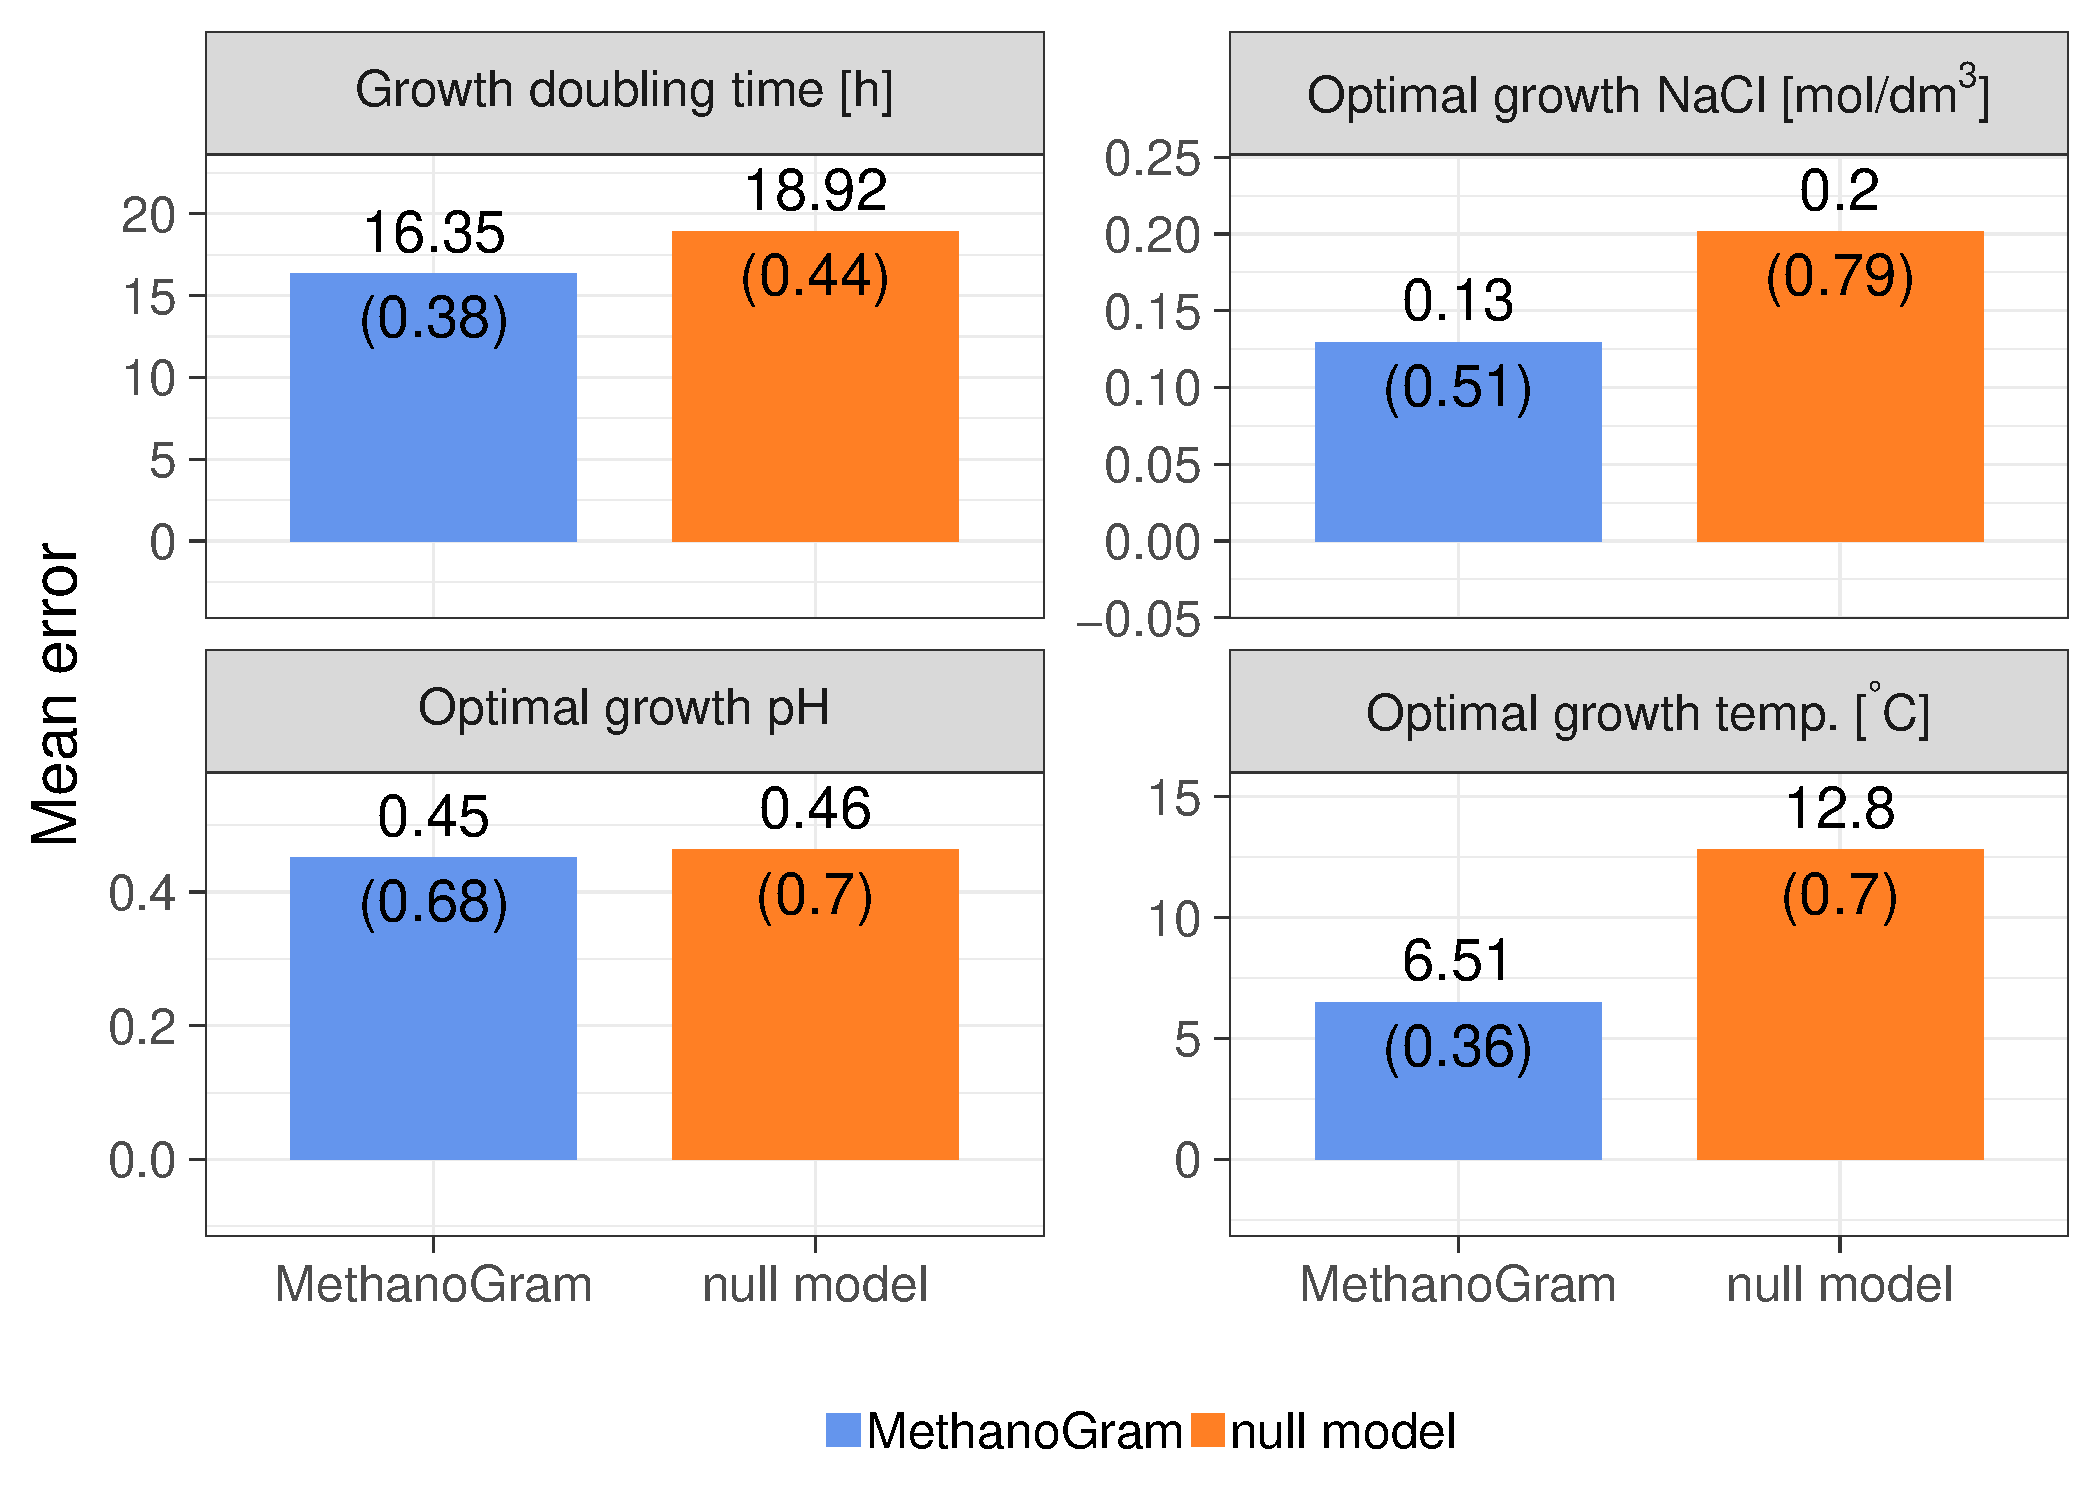
\includegraphics[width=\maxwidth]{figure/unnamed-chunk-1-1} 
% 
% }
% 
% 
% 
% \end{knitrout}

PhyMet$^2$ (Phylogeny and Metabolism of Methanogens) is the largest data analysis platform that provides information on culturing conditions and sequence data for methanogenic archaea with a user-friendly interface. The analyses include advanced data browsing, exploring phylogeny, plotting selected features, searching for potential sequence homologues and predicting key culturing conditions for newly discovered methanogens based on 16S rRNA sequences.


% \normalsize	
% \bigskip
% 
% \bigskip
% 
% \bigskip

\end{block}
\vfill


% \begin{block}{Quick Permutation Test (QuiPT)}
%     Model and statistic independent permutation tests can be used to filter features obtained through counting n-grams.
%     
%     During a permutation test class labels are randomly exchanged during computation of a significance statistic. p-values are defined as:
%     
% \begin{center}
% \scalebox{0.85}{
% $      
% \textnormal{p-value} = \frac{N_{T_P > T_R}}{N}
% $
% }
% \end{center}
% 
% where $N_{T_P > T_R}$ is number of times when $T_P$ (permuted test statistic) was more extreme than $T_R$ (test statistic for non-permuted data).
% 
% Permutation tests are computationally expensive (especially considering precise estimation of small p-values, because the number of permutations is inversely proportional to the interval between p-values).
% 
% \medskip
% 
% \textbf{Qui}ck \textbf{P}ermutation \textbf{T}est (QuiPT) thanks to the unique parameterization replaces a permutation test with the exact two-sided Fisher's test~\citep{lehmann1986testing} reducing the computation cost. 
%       
%     \end{block}

\vfill

\begin{block}{MethanoGram}
% \begin{knitrout}
% \definecolor{shadecolor}{rgb}{0.969, 0.969, 0.969}\color{fgcolor}
% 
% {\centering \includegraphics[width=\maxwidth]{figure/unnamed-chunk-2-1} 
% 
% }
% 
% 
% 
% \end{knitrout}

% From metagenomics analyses, we know that there is a plethora of new uncultivated microorganisms, including methanogens. Unfortunately, we can often cultivate much less species than actually occur in a given environment.\\
The unique feature of PhyMet2 is a web server, MethanoGram, that predicts conditions for the optimal growth of methanogens: temperature, pH, NaCl concentration, and growth doubling time.

% The data contained in PhyMet2 was used to develop a web server, MethanoGram, that quickly and accurately predicts the conditions for optimal growth of methanogens: temperature, pH, and NaCl concentration, i.e. the key factors that shape the composition of methanogenic communities.\\
% MethanoGram is able to estimate:
% 
% \begin{multicols}{2}
% \begin{itemize}
% \item{growth doubling time}
% \item{optimal growth temperature}
% \item{optimal growth pH}
% \item{optimal growth NaCl}
% \end{itemize}
% \end{multicols}

% The prediction of culturing conditions is performed by the web server MethanoGram based on 16S rRNA. 

MethanoGram is one of the first approaches aiming at predicting the phenotype of microorganisms based on molecular markers, and hopefully will boost further research in the field. We would also like to apply our algorithm to prediction of culturing conditions for other microorganisms.

% Therefore we have created MethanoGramm which is one of first approches to predict culturing conditions of methanogens.

\end{block}


}
\end{minipage}
\end{beamercolorbox}
\end{column}


%new column ------------------------------------------------------    

\begin{column}{.48\textwidth}
\begin{beamercolorbox}[center,wd=\textwidth]{postercolumn}
\begin{minipage}[T]{.95\textwidth}  
\parbox[t][\columnheight]{\textwidth}
{





% \vfill



\begin{block}{Tuning of MethanoGram}

In order to train MethanoGram, we used n-grams, i.e. subsequences of the length n that were extracted from 16S rRNA. We chose only those species that have known 16S rRNA as well as all important culturing conditions. 

\begin{figure}
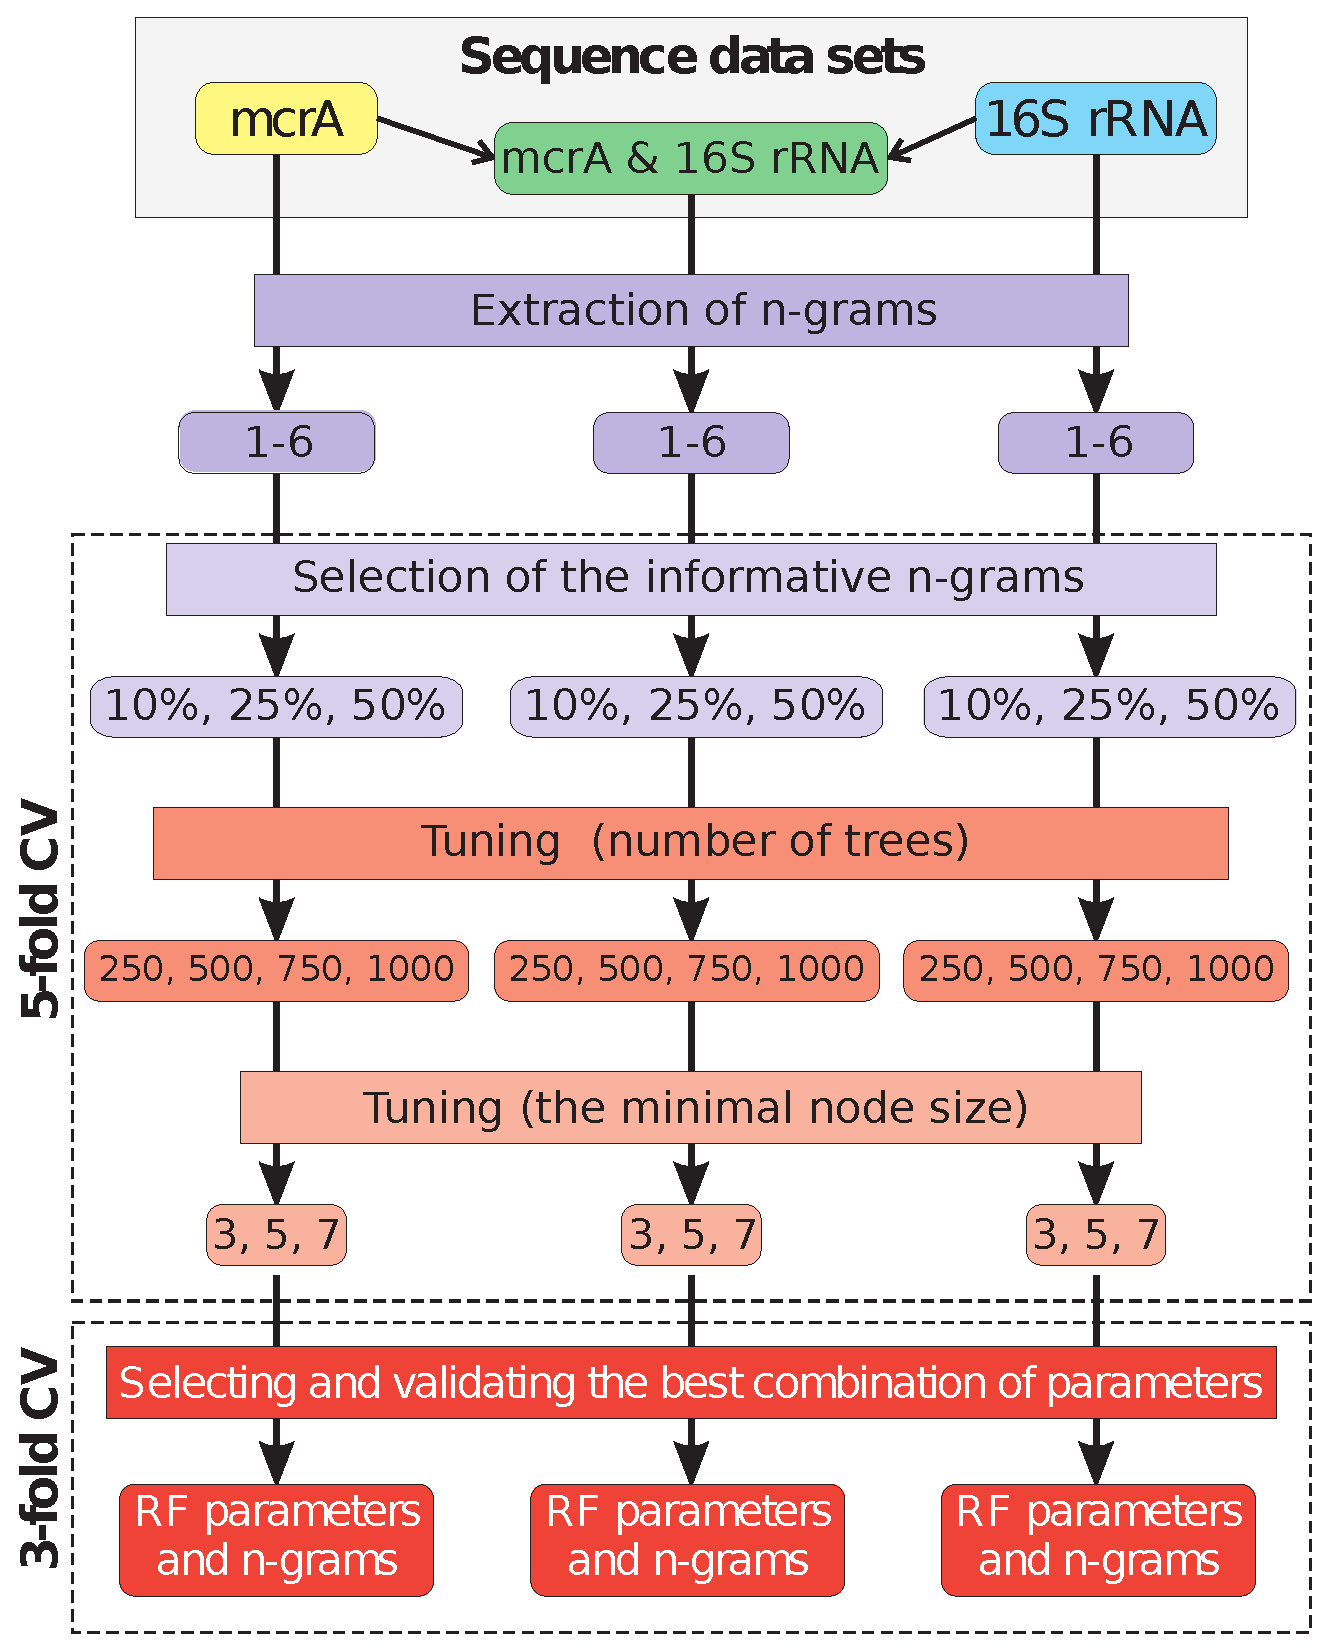
\includegraphics[width=0.75\columnwidth]{suplem2.eps}
\end{figure}


To estimate the culturing conditions we implemented random forests algorithm and performed a nested cross-validation.

\end{block}
% \vfill


\begin{block}{Mean error}


\begin{knitrout}
\definecolor{shadecolor}{rgb}{0.969, 0.969, 0.969}\color{fgcolor}

{\centering 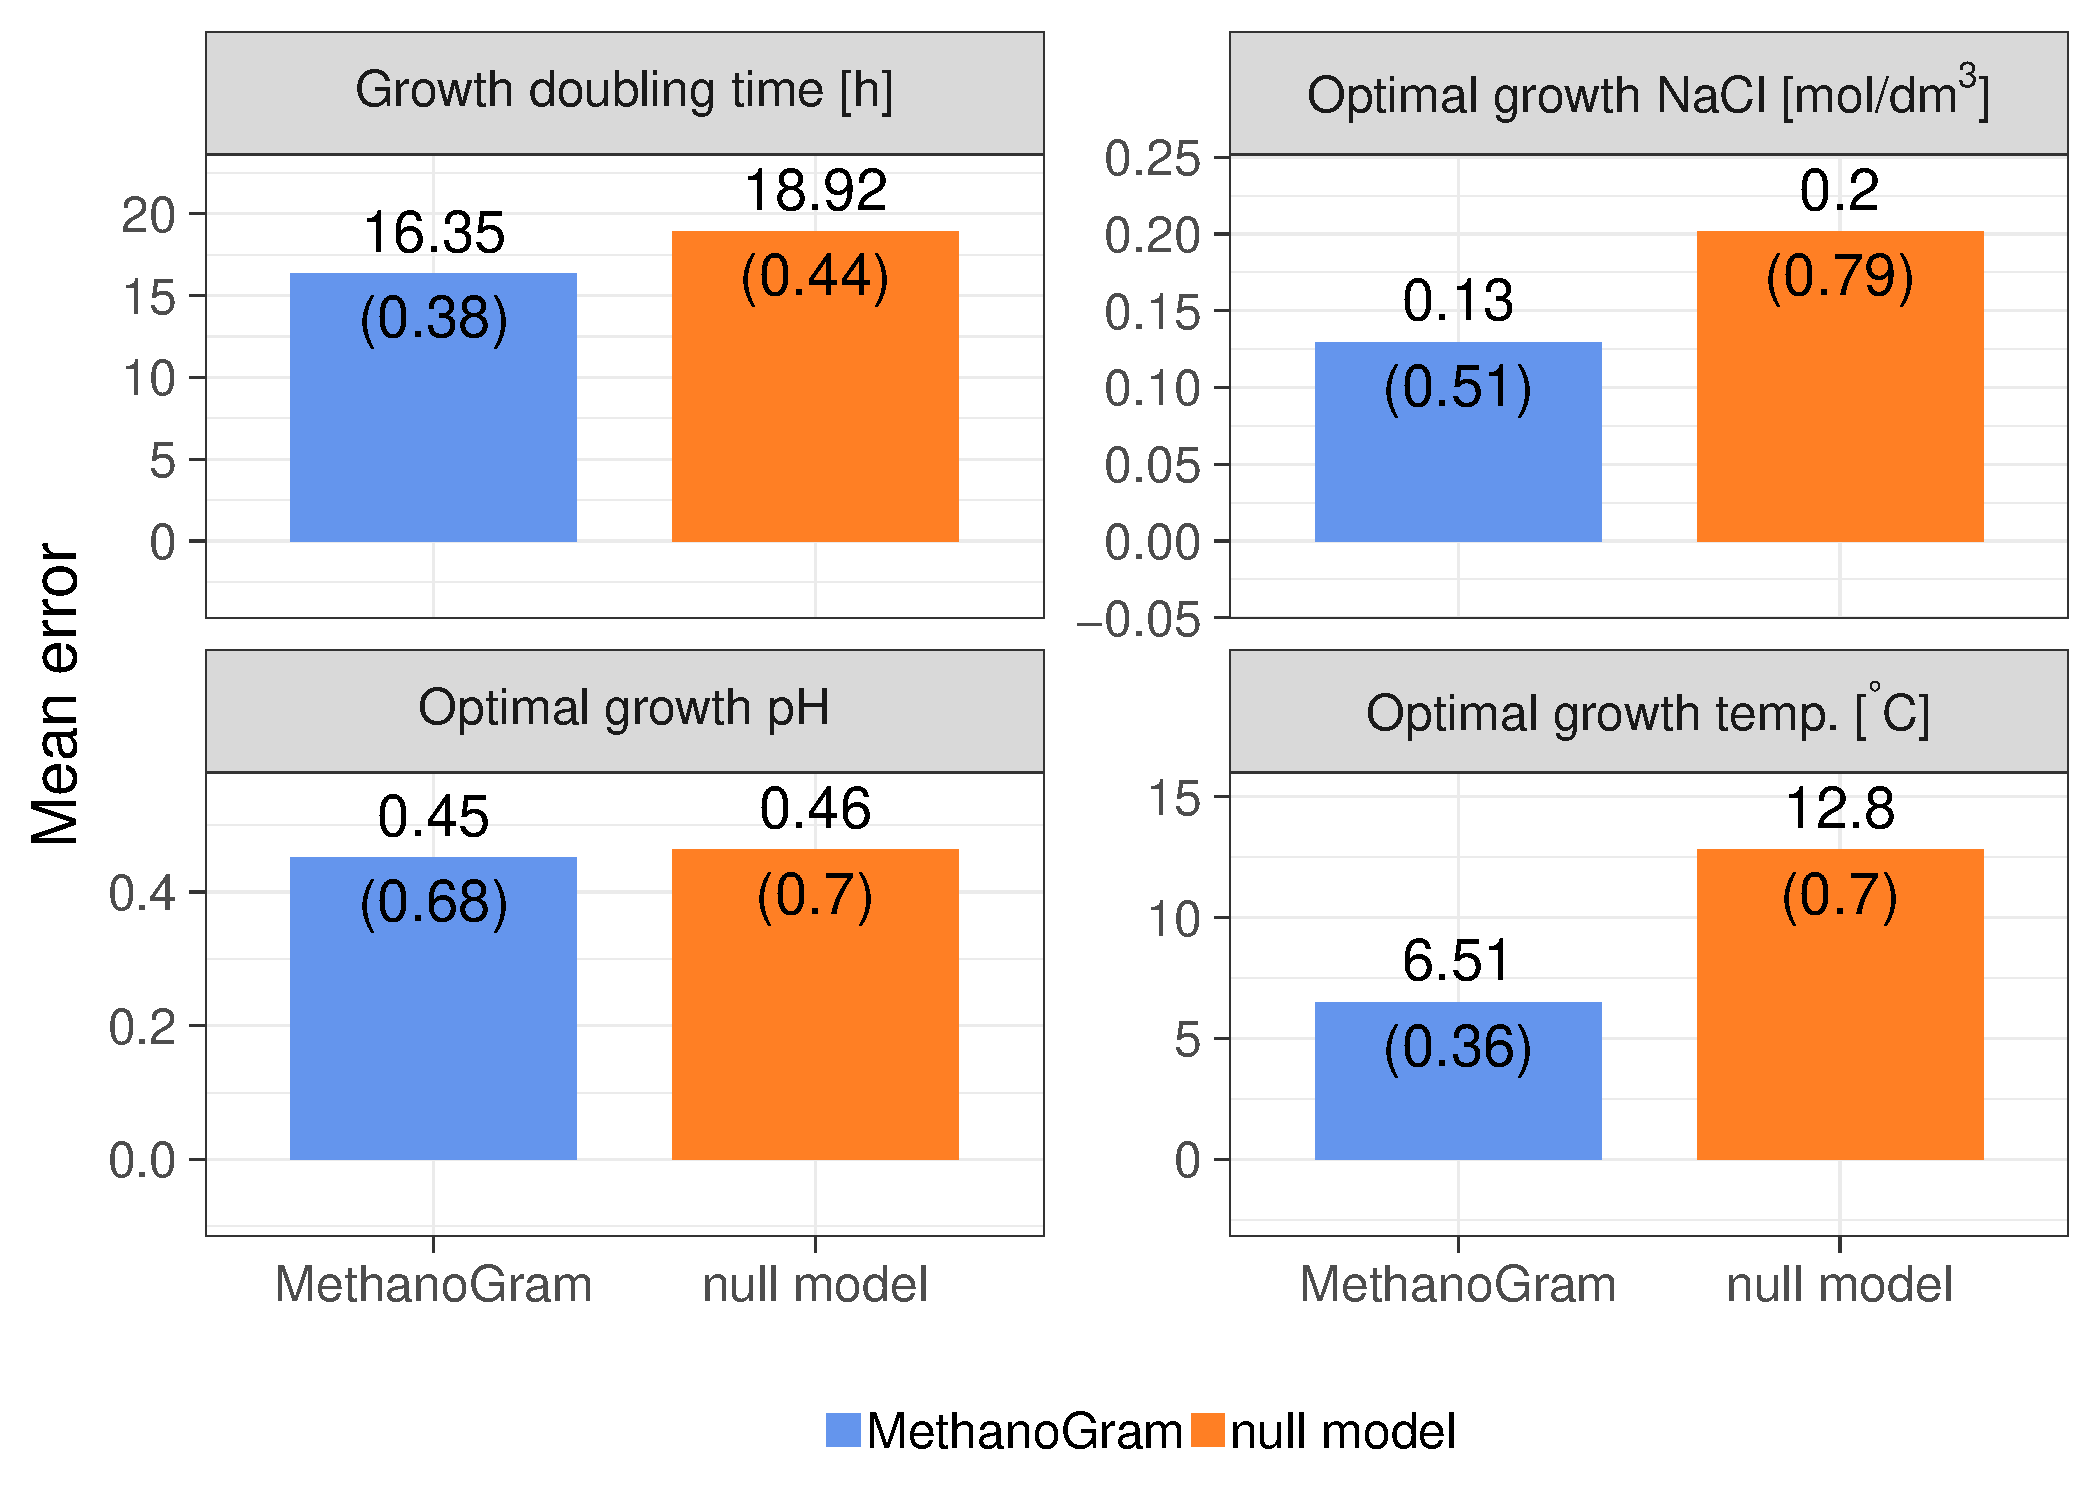
\includegraphics[width=\maxwidth]{figure/unnamed-chunk-1-1} 

}



\end{knitrout}

% \begin{knitrout}
% \definecolor{shadecolor}{rgb}{0.969, 0.969, 0.969}\color{fgcolor}
% 
% {\centering \includegraphics[width=\maxwidth]{figure/unnamed-chunk-3-1} 
% 
% }
% 
% 
% 
% \end{knitrout}

Null model does not incorporate any sequence-based information. \\
Values above columns represent mean error of algorithm, below show mean errors of the best predictors found in the nested cross-validation.


\end{block}
\vfill


\begin{block}{Funding and aviability}

PhyMet$^2$ is avaible at: \url{http://metanogen.biotech.uni.wroc.pl/}.

\bigskip

MethanoGram is avaible as a web-server: \url{http://www.smorfland.uni.wroc.pl/shiny/mgp/}.

\bigskip

The exact details on training of MethanoGram are accessible at: \url{https://github.com/michbur/PhyMet2_supplements}.
% \vfill
\bigskip


\small{This work was supported by the Leading National Research Center (KNOW) and the National Science Centre grant no. 2015/17/N/NZ2/01845 and 2017/24/T/NZ2/00003.}
\nocite{jablonski_methanogenic_2015}


\end{block}
\vfill

 \begin{block}{Bibliography}
  \tiny{
  \bibliographystyle{apalike}
  \bibliography{references}
  }
  \end{block}
  \vfill  


}
\end{minipage}
\end{beamercolorbox}
\end{column}
\end{columns}  
\end{frame}
\end{document}
